\subsubsection{User application -- Java Swing}
\label{subsubsec:client-user}

The V1 user interface is built with Java Swing on Windows, for managing the
account, connecting with friends and exchanging messages. The subsystem of the
functions in this table is User. Function codes are independent of task codes and
of the order in which the report presents them.

\begingroup
\small
\begin{longtable}{|C{1.2cm}|L{\dimexpr\textwidth-1.2cm-4\tabcolsep-3\arrayrulewidth\relax}|}
  \caption{Functions of the user subsystem}
  \label{tab:user-features}\\
  \hline
  \textbf{Code} & \textbf{Function and scope}\\
  \hline
  \endfirsthead
  \hline
  \textbf{Code} & \textbf{Function and scope}\\
  \hline
  \endhead
  \hypertarget{F01}{\texttt{F01}} & \textbf{Register an account.}\\
  \hline
  \hypertarget{F02}{\texttt{F02}} & \textbf{Sign in.}\\
  \hline
  \hypertarget{F03}{\texttt{F03}} &
  \textbf{Update account information:} the profile editing interface, with the
  fields that match the user profile in \hyperlink{F13}{F13}.\\
  \hline
  \hypertarget{F04}{\texttt{F04}} &
  \textbf{Reset password:} generate a random password and send it by email.\\
  \hline
  \hypertarget{F05}{\texttt{F05}} & \textbf{Change password.}\\
  \hline
  \hypertarget{F06}{\texttt{F06}} &
  \textbf{Manage friends:} show the list, filter by name and see online/offline
  status; find people and send friend requests; unfriend; block and unfriend at once
  so the blocked person cannot send a request again.\\
  \hline
  \hypertarget{F07}{\texttt{F07}} &
  \textbf{Handle friend requests:} show, filter by name, accept or decline.\\
  \hline
  \hypertarget{F08}{\texttt{F08}} &
  \textbf{View online friends:} filter by name, start a chat or create a group.\\
  \hline
  \hypertarget{F09}{\texttt{F09}} &
  \textbf{Find people:} search by name or username, never showing people who
  blocked you; from the results, start a chat or create a group.\\
  \hline
  \hypertarget{F10}{\texttt{F10}} &
  \textbf{Report spam:} report an unwanted message received from someone.\\
  \hline
  \hypertarget{F11}{\texttt{F11}} &
  \textbf{Private chat and history:} real-time messaging when online; messages are
  kept for offline people to read later; view the history, delete all of it or some
  messages; search one or all conversations and jump to the result; call an LLM to
  rewrite or suggest messages.\\
  \hline
  \hypertarget{F12}{\texttt{F12}} &
  \textbf{Group chat:} create a group with at least one other username, rename it,
  add members, make members group admins, chat and encrypt the group; only group
  admins can remove members.\\
  \hline
\end{longtable}
\endgroup

In V1, this list is used to check the user screens against the requirements.
Sending messages, sending email, calling an LLM and group encryption do not have to
work yet at this stage; the preview only simulates their results with in-memory
sample data.

\paragraph{Navigation and screen list}
\label{par:user-navigation}
\mbox{}\par
When the V1 preview starts, the application opens the \textbf{Sign in} screen,
separate from \textbf{Admin Sign in}. From there the user can go to \textbf{Register}
or \textbf{Forgot password}. After signing in, the left sidebar is split into
\textbf{Messages} (\textbf{Chat}, \textbf{Group}), \textbf{People}
(\textbf{Friend}) and \textbf{Settings} (\textbf{Account}); the \textbf{Chat} screen
opens first. Each function lives on exactly one screen; other screens only link to
it. For example, the \textbf{Chat} button on the \textbf{Friend} page opens the
conversation on the \textbf{Chat} page, and the \textbf{Create group} button opens
the \textbf{Group} page's create form with the selected members.
Table~\ref{tab:user-screen-map} maps the Swing interface to the Figma prototype~\cite{ref:figma} and
to the function codes of the assignment. Labels in the table are quoted from the
interface.

\begingroup
\small
\begin{longtable}{|L{4.3cm}|L{\dimexpr\textwidth-4.3cm-4\tabcolsep-3\arrayrulewidth\relax}|}
  \caption{V1 user screens}
  \label{tab:user-screen-map}\\
  \hline
  \textbf{Screen} & \textbf{Functions and content}\\
  \hline
  \endfirsthead
  \hline
  \textbf{Screen} & \textbf{Functions and content}\\
  \hline
  \endhead
  \href{https://www.figma.com/design/maCogjZs9eOOhfkxsOZoIU?node-id=129-929}{Sign in}
  & \hyperlink{F02}{F02}. Username, password, the \textbf{Forgot password?} and
  \textbf{Create account} links. Error messages when a field is empty, when the
  username or password is wrong, and when an administrator has locked the account
  (\hyperlink{F13}{F13}).\\
  \hline
  \href{https://www.figma.com/design/maCogjZs9eOOhfkxsOZoIU?node-id=129-929}{Register}
  & \hyperlink{F01}{F01}. Username, full name, email, gender, date of birth and
  address (both optional), password and confirmation. Every invalid field is marked
  at once: username or email already used, invalid email or date of birth, password
  shorter than 8 characters or not matching. The new account is signed in right
  away.\\
  \hline
  \href{https://www.figma.com/design/maCogjZs9eOOhfkxsOZoIU?node-id=129-929}{Forgot password}
  & \hyperlink{F04}{F04}. Enter the account's email; the system generates a random
  password and sends it by email. V1 shows the email content inside the app; real
  email sending comes in V2.\\
  \hline
  \href{https://www.figma.com/design/maCogjZs9eOOhfkxsOZoIU?node-id=129-930}{Chat}
  & \hyperlink{F10}{F10}, \hyperlink{F11}{F11}, \hyperlink{F12}{F12} (group chat).
  One list for private and group conversations, with a name filter, an online dot
  and a lock icon for encrypted groups. My last message shows \textbf{Sent} when the
  server has it (group messages), \textbf{Waiting} when the recipient is offline and
  \textbf{Delivered} when the recipient has it: at once if they are online, or when
  they sign in again. The status is derived from \texttt{Message.deliveredAt}.
  Select one or more messages to \textbf{Delete for me} or \textbf{Report spam} (only
  one received message not reported yet, with a reason); \textbf{Clear history}
  clears the whole history for the current user only. \textbf{Search in chat} and
  \textbf{Search all messages} search one or all conversations and jump to the
  message. \textbf{Suggest} and \textbf{Improve} call the AI assistant to suggest or
  rewrite a message; both are refused in encrypted groups because the assistant may
  not read encrypted content. A chat with someone I blocked, someone who blocked me,
  or an account locked by an administrator (\hyperlink{F13}{F13}) shows a
  \textbf{Blocked} or \textbf{Locked} label and replaces the message box with an
  explanation.\\
  \hline
  \href{https://www.figma.com/design/maCogjZs9eOOhfkxsOZoIU?node-id=129-931}{Group}
  & \hyperlink{F12}{F12}. Group list with a name and role filter.
  \textbf{Create group} needs a group name and at least one other username.
  A group always has at least two people, so a member cannot be removed when only two
  are left. The group detail has \textbf{Rename}, \textbf{Add member},
  \textbf{Open chat} and the member table. \textbf{Make admin}, \textbf{Remove} and the
  \textbf{Encrypted group} toggle work only for group admins; for other members they
  are disabled with an explanation. A member whose account is locked carries the
  \textbf{Locked} label: a group admin can only \textbf{Remove} them, not
  \textbf{Make admin} them or add the account again. A removed member is recorded with
  \texttt{leftAt}, so their earlier messages stay in the history.\\
  \hline
  \href{https://www.figma.com/design/maCogjZs9eOOhfkxsOZoIU?node-id=129-932}{Friend}
  & \hyperlink{F06}{F06}--\hyperlink{F09}{F09}. \textbf{Friends} tab: name filter,
  online/offline status, \textbf{Chat}, \textbf{Unfriend}, \textbf{Block}.
  \textbf{Online} tab: online friends, select several people to create a group.
  \textbf{Requests} tab: accept or decline received requests, see sent requests.
  \textbf{Find people} tab: search by name or username, never showing people who
  blocked you; actions depend on the relationship (\textbf{Add friend},
  \textbf{Accept}, \textbf{Chat}, \textbf{Create group}, \textbf{Block}). A blocked
  person cannot send a friend request. A locked account carries the \textbf{Locked}
  label and accepts no actions: a locked friend only has \textbf{Unfriend}, a request
  from a locked account only has \textbf{Decline}, and \textbf{Find people} shows no
  buttons for it.\\
  \hline
  \href{https://www.figma.com/design/maCogjZs9eOOhfkxsOZoIU?node-id=129-933}{Account}
  & \hyperlink{F03}{F03}, \hyperlink{F05}{F05}. Profile card; \textbf{Edit profile}
  updates the full name, email, gender, date of birth and address; the username cannot
  be changed. \textbf{Change password} asks for the current password, the new password
  and its confirmation. \textbf{Sign Out} in the sidebar returns to the sign-in
  screen.\\
  \hline
\end{longtable}
\endgroup

\paragraph{V1 Java Swing screenshots}
\mbox{}\par
The screenshots below are captured from the Java Swing application in the
\texttt{user-client} module running on in-memory sample data. The signed-in sample
user is \textbf{Maya Chen}: sign in with the username \texttt{mayachen} and the
password \texttt{chatapp123}; every sample account shares this password, and
\texttt{linhng}, \texttt{owentran} and \texttt{ryanh} are locked. The sample data is
the same as in the administrator application. Changes last only for the preview
session. Real-time messaging, sending email, the AI assistant and group encryption
are simulated: the results look as designed, but there is no real server, email or
LLM yet.

\noindent\begin{minipage}{\linewidth}
  \centering
  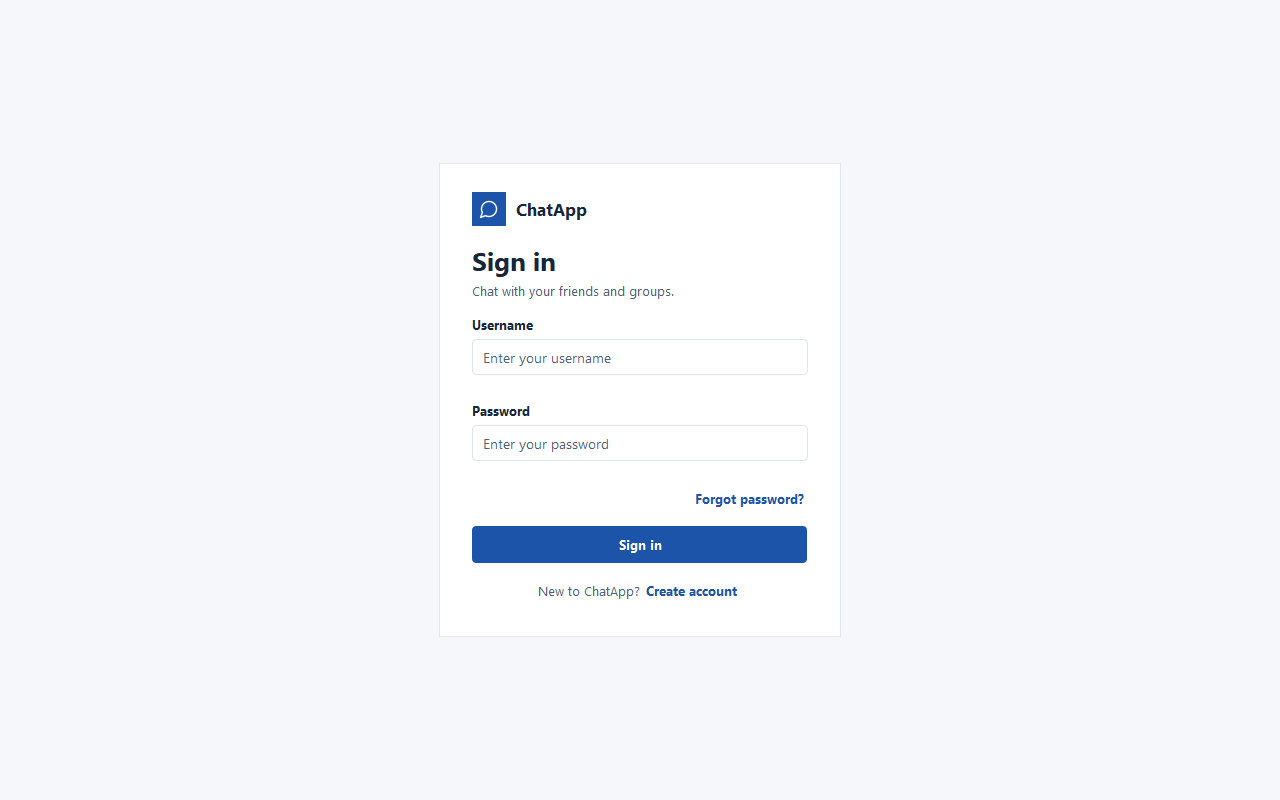
\includegraphics[width=.48\linewidth]{images/user-swing-login.png}\hfill
  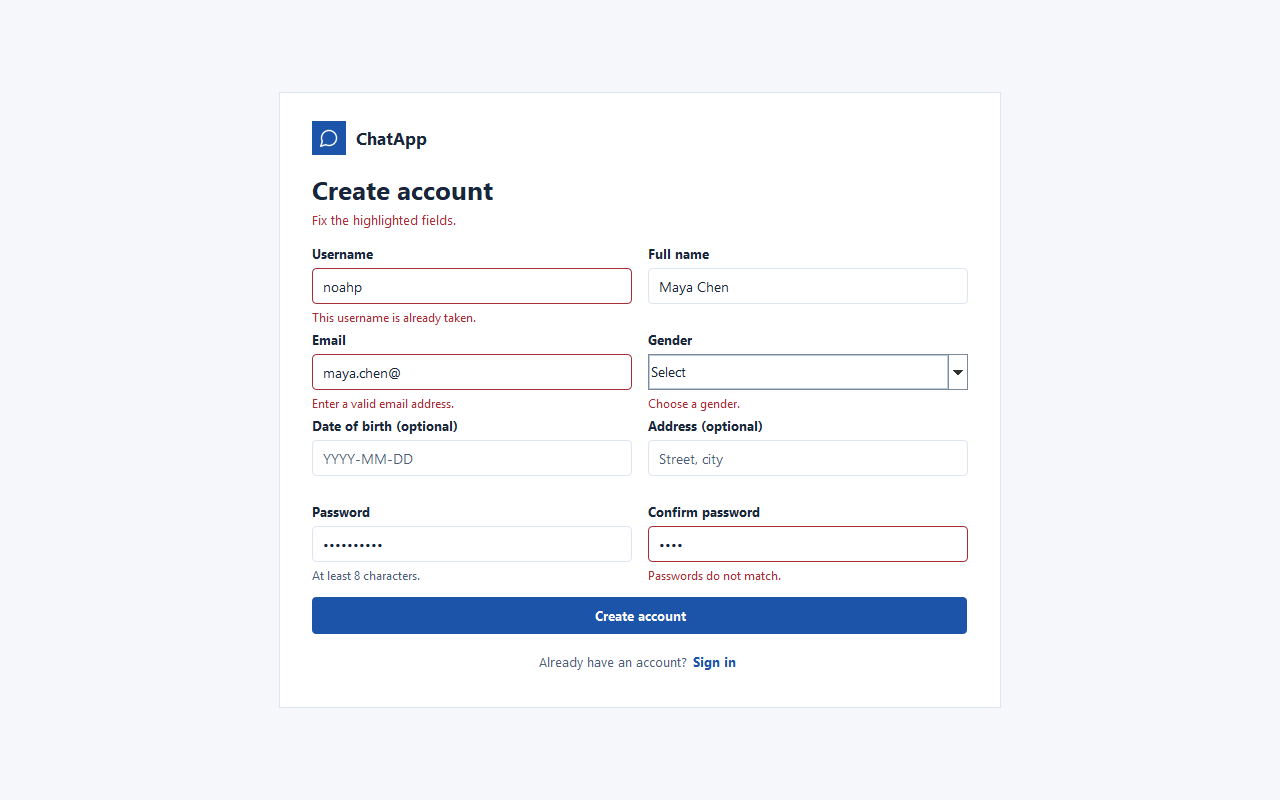
\includegraphics[width=.48\linewidth]{images/user-swing-register.png}
  \captionof{figure}{F02 and F01. Sign in and register, with input checks.}
  \label{fig:user-swing-login-register}
\end{minipage}

\noindent\begin{minipage}{\linewidth}
  \centering
  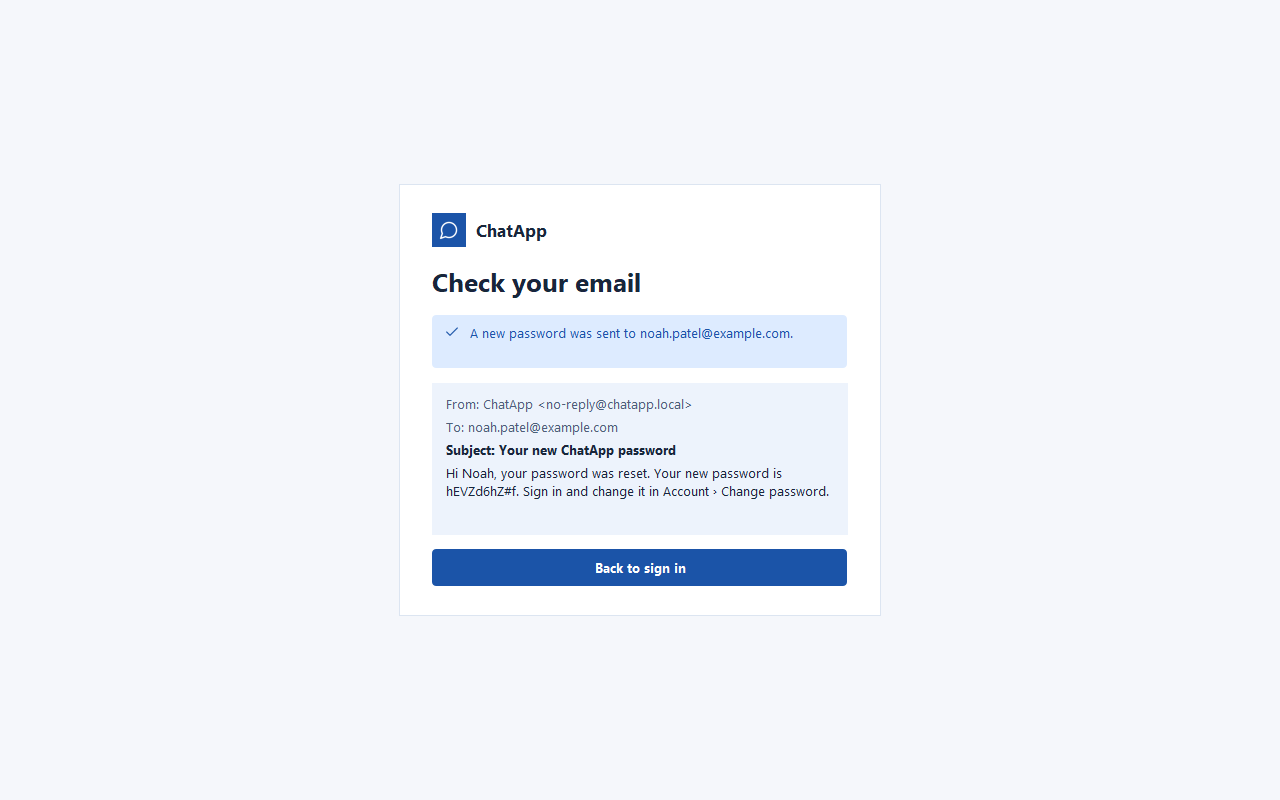
\includegraphics[width=.74\linewidth]{images/user-swing-forgot-password.png}
  \captionof{figure}{F04. The new random password and the email sent to the user.}
  \label{fig:user-swing-forgot-password}
\end{minipage}

\noindent\begin{minipage}{\linewidth}
  \centering
  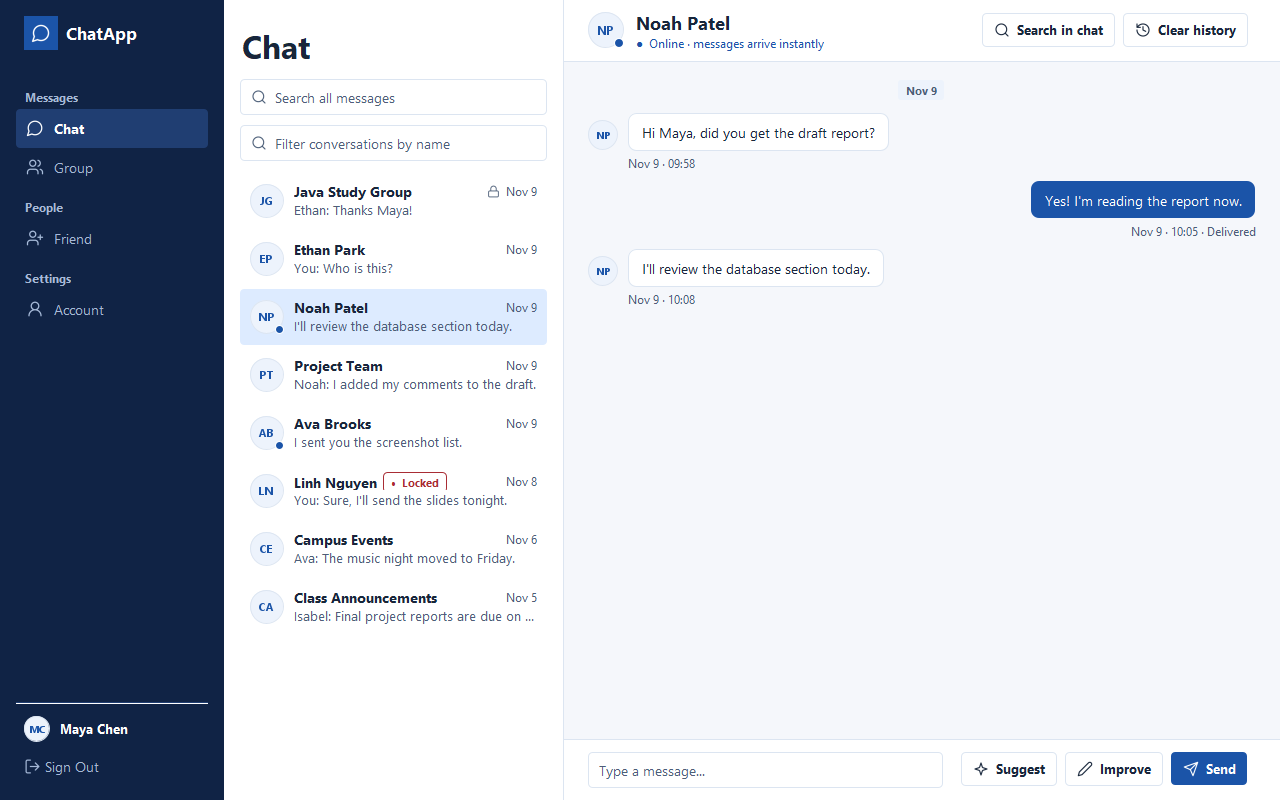
\includegraphics[width=.48\linewidth]{images/user-swing-chat.png}\hfill
  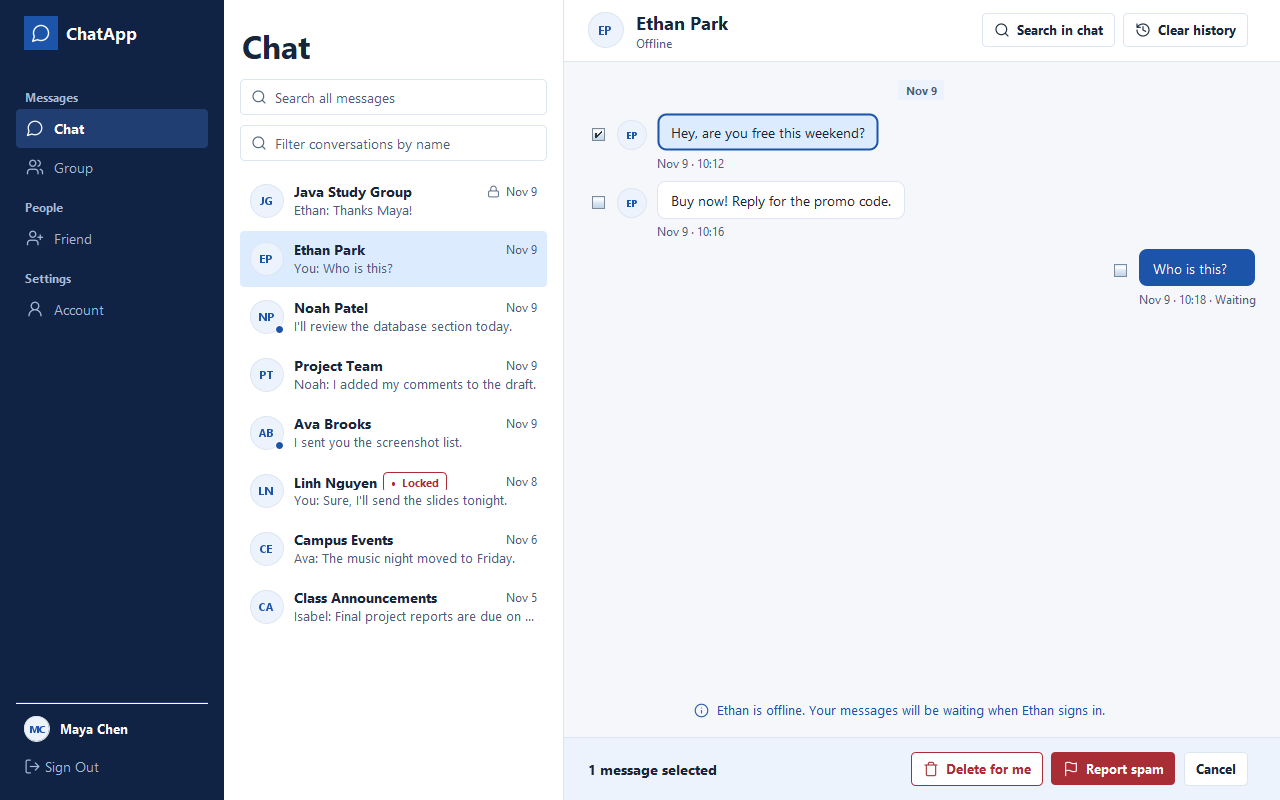
\includegraphics[width=.48\linewidth]{images/user-swing-chat-select.png}
  \captionof{figure}{F11 and F10. Chat with an online friend, message Delivered; select messages to delete for yourself or report spam; a message to an offline friend stays Waiting until that person signs in.}
  \label{fig:user-swing-chat}
\end{minipage}

\noindent\begin{minipage}{\linewidth}
  \centering
  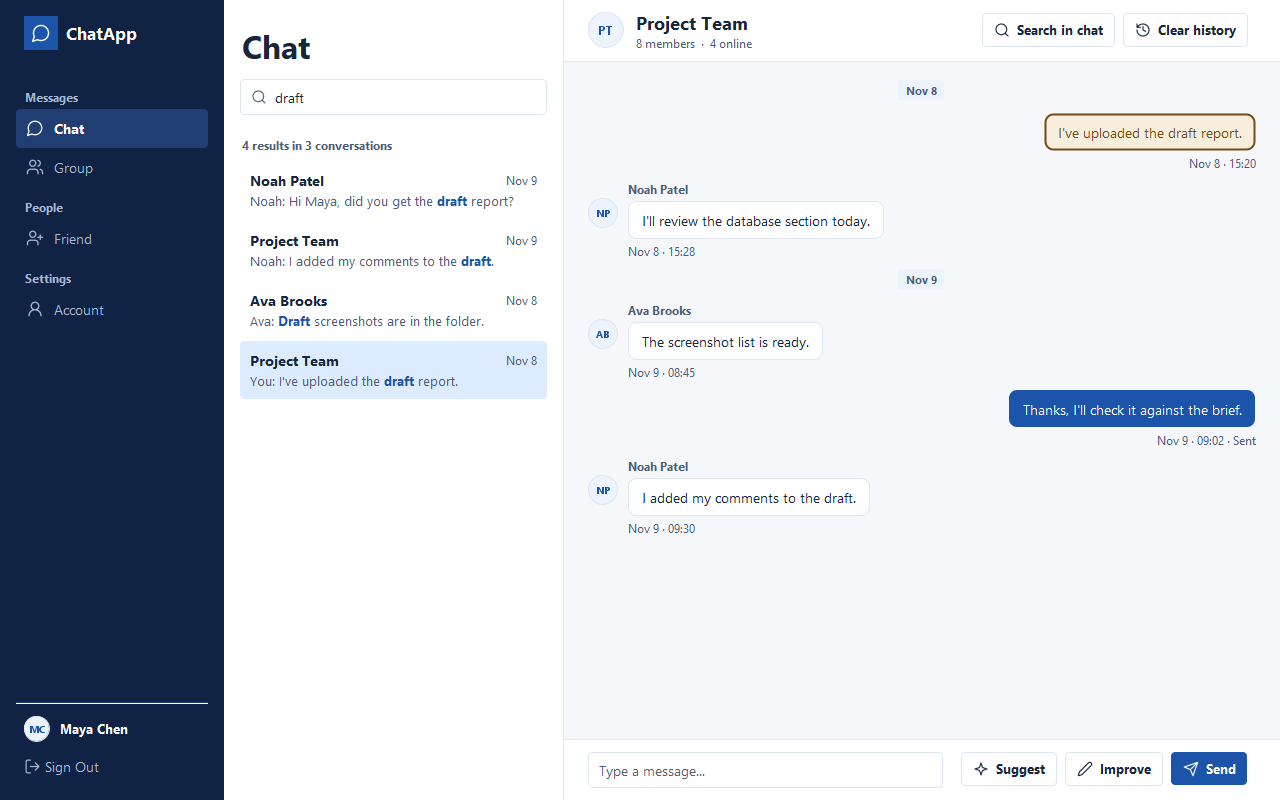
\includegraphics[width=.48\linewidth]{images/user-swing-chat-search.png}\hfill
  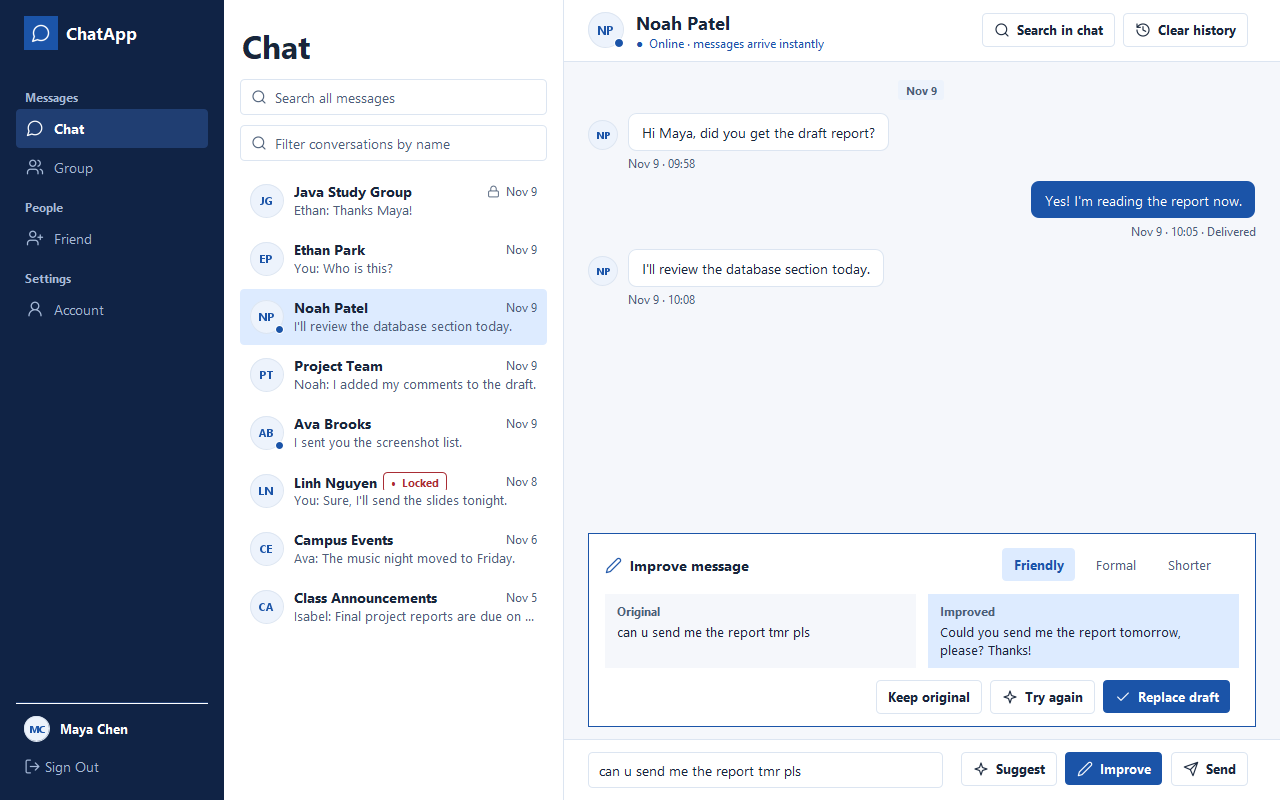
\includegraphics[width=.48\linewidth]{images/user-swing-chat-llm.png}
  \captionof{figure}{F11. Search all conversations and jump to the message; the AI assistant rewrites a message.}
  \label{fig:user-swing-chat-search-llm}
\end{minipage}

\noindent\begin{minipage}{\linewidth}
  \centering
  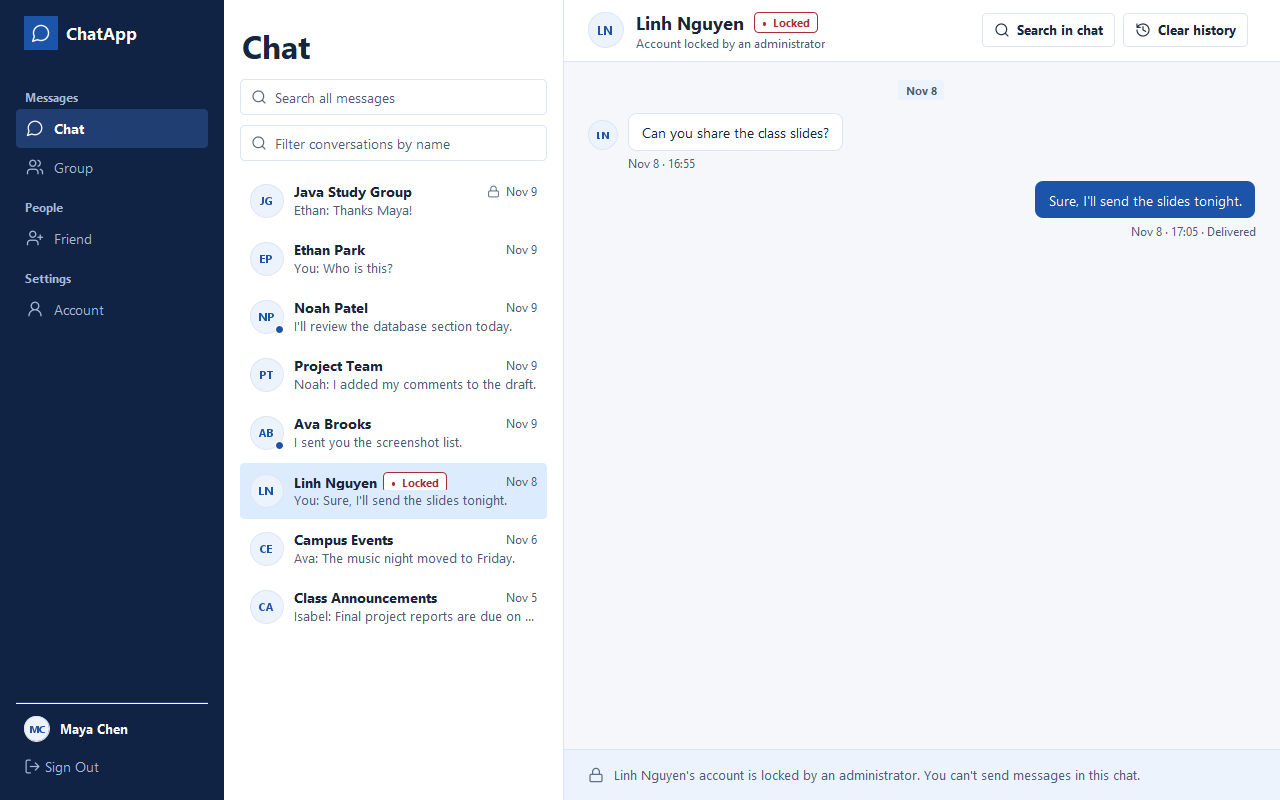
\includegraphics[width=.74\linewidth]{images/user-swing-chat-locked.png}
  \captionof{figure}{F11 and F13. A chat with an account locked by an administrator: Locked label, no sending.}
  \label{fig:user-swing-chat-locked}
\end{minipage}

\noindent\begin{minipage}{\linewidth}
  \centering
  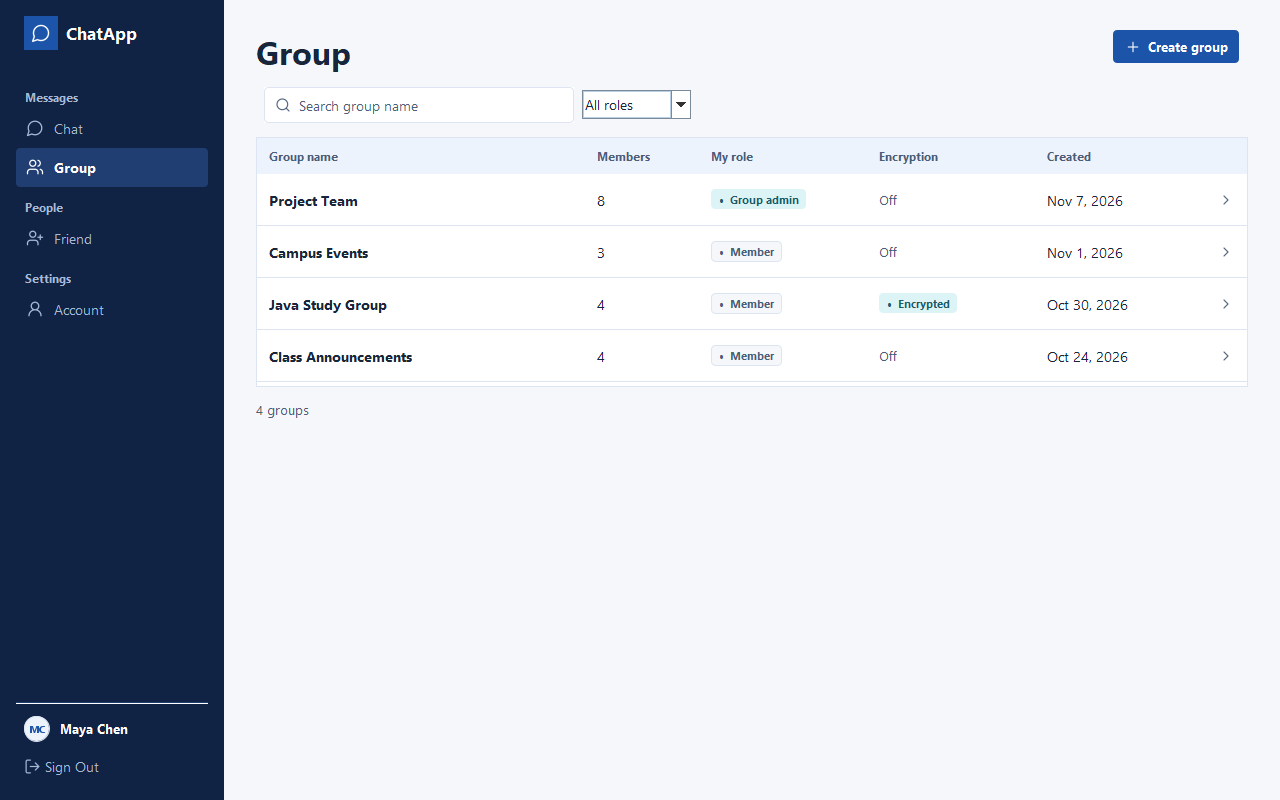
\includegraphics[width=.48\linewidth]{images/user-swing-group.png}\hfill
  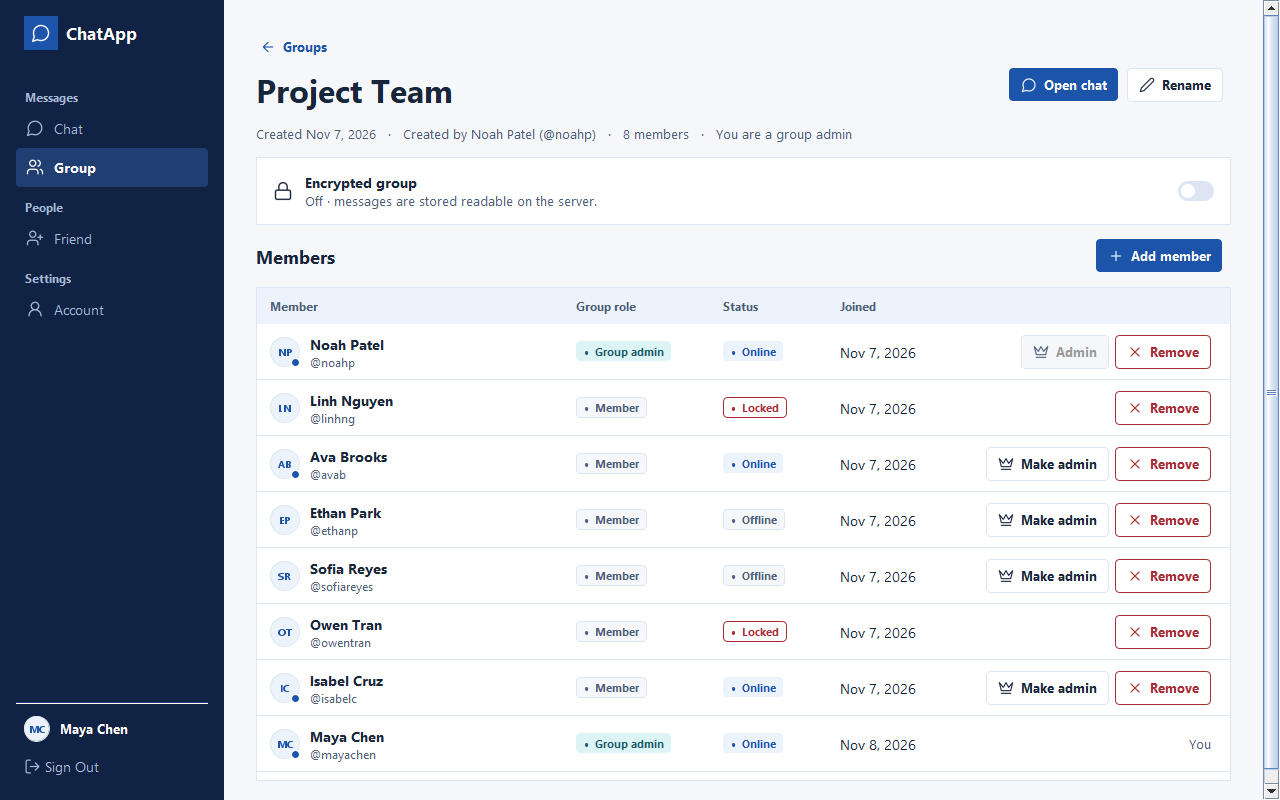
\includegraphics[width=.48\linewidth]{images/user-swing-group-detail.png}
  \captionof{figure}{F12. Group list and group detail with group admin rights; a locked member can only be removed.}
  \label{fig:user-swing-group}
\end{minipage}

\noindent\begin{minipage}{\linewidth}
  \centering
  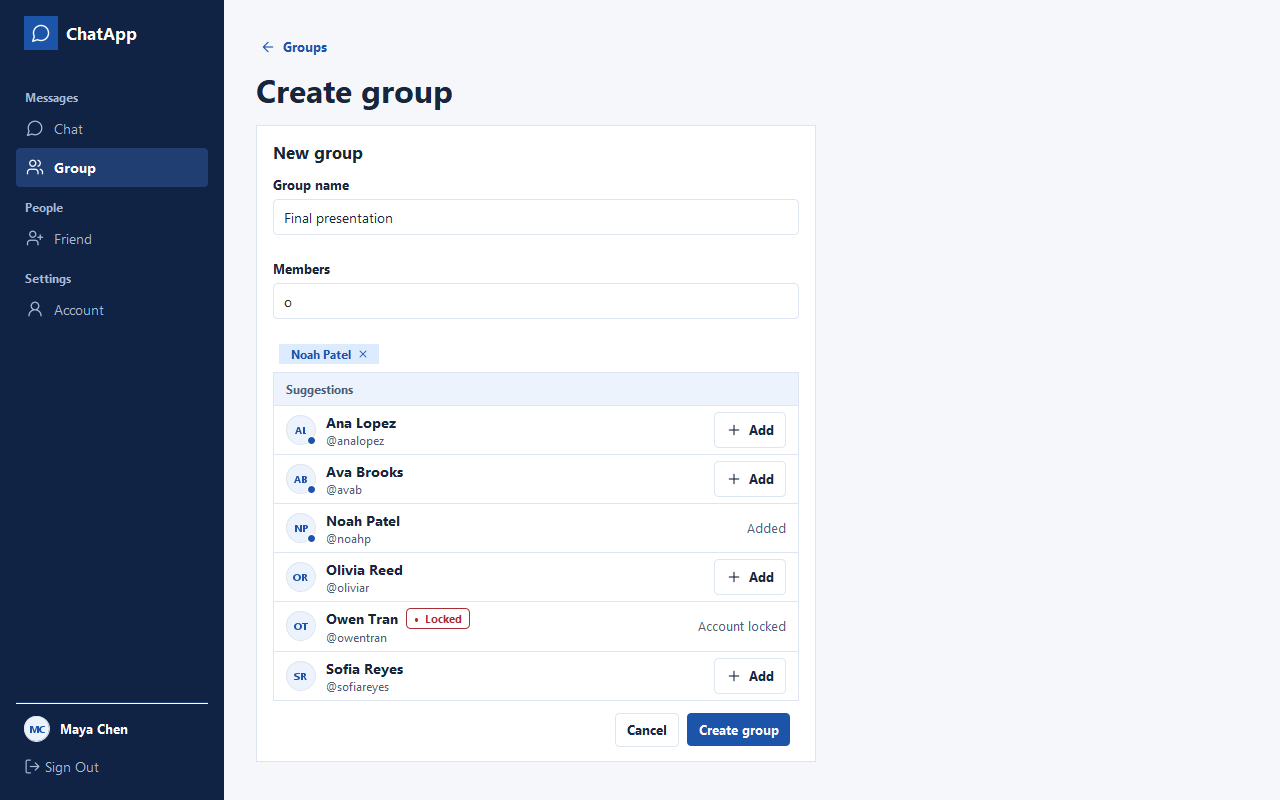
\includegraphics[width=.74\linewidth]{images/user-swing-group-create.png}
  \captionof{figure}{F12. Create a group with at least one other username.}
  \label{fig:user-swing-group-create}
\end{minipage}

\noindent\begin{minipage}{\linewidth}
  \centering
  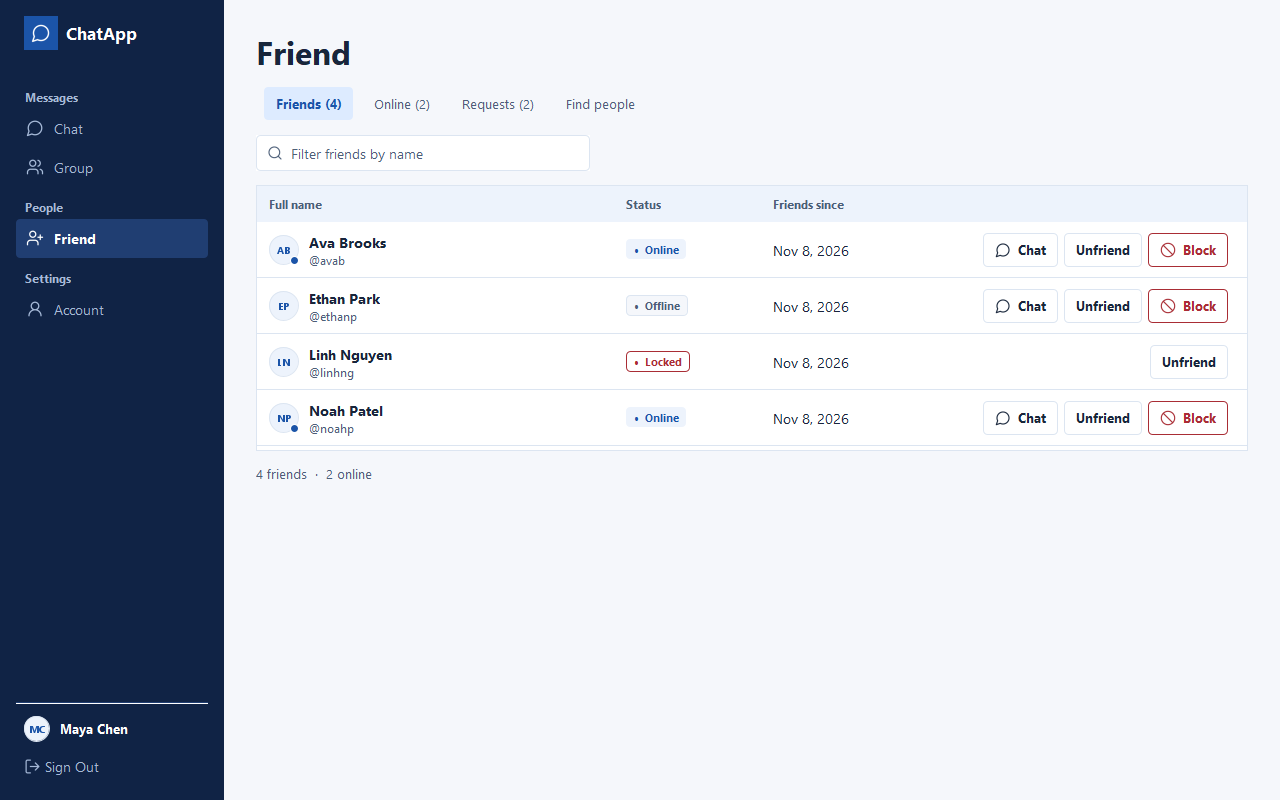
\includegraphics[width=.48\linewidth]{images/user-swing-friend.png}\hfill
  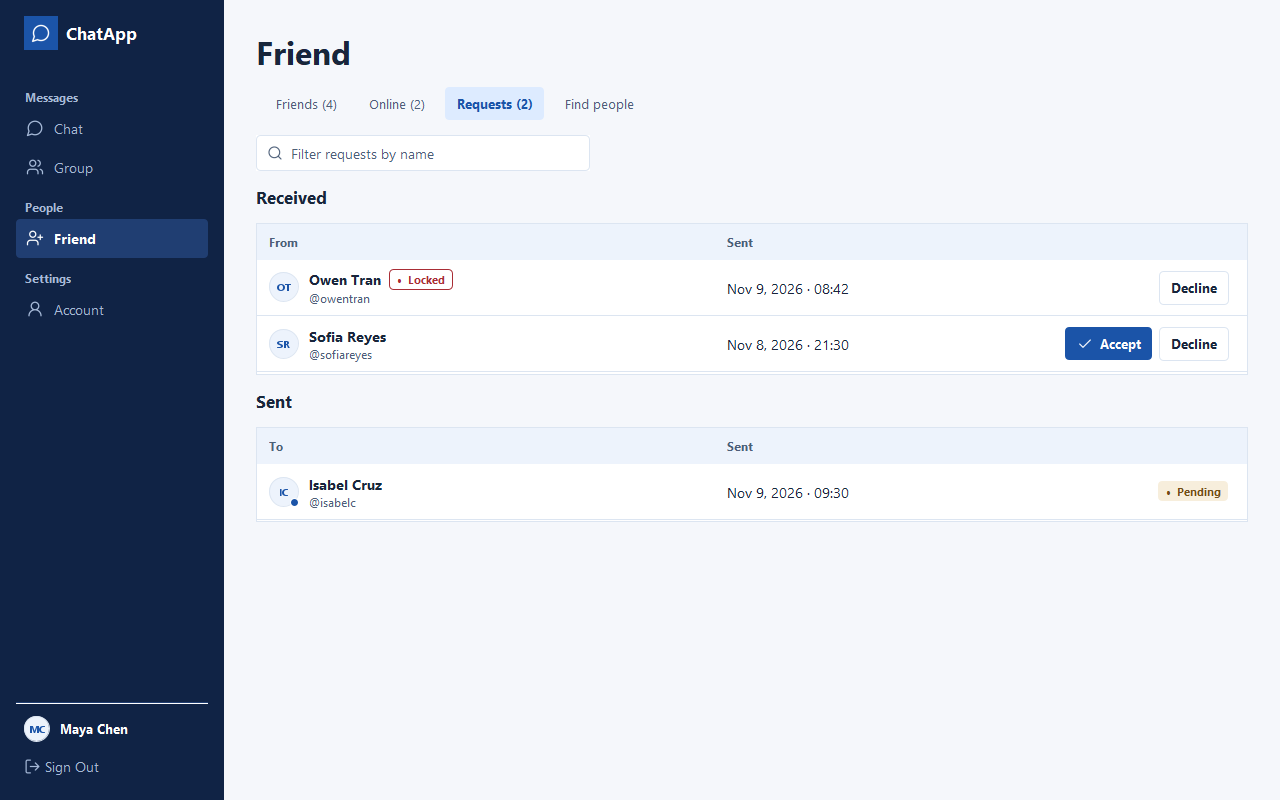
\includegraphics[width=.48\linewidth]{images/user-swing-friend-requests.png}
  \captionof{figure}{F06 and F07. Friend list and friend requests; locked accounts carry the Locked label.}
  \label{fig:user-swing-friend}
\end{minipage}

\noindent\begin{minipage}{\linewidth}
  \centering
  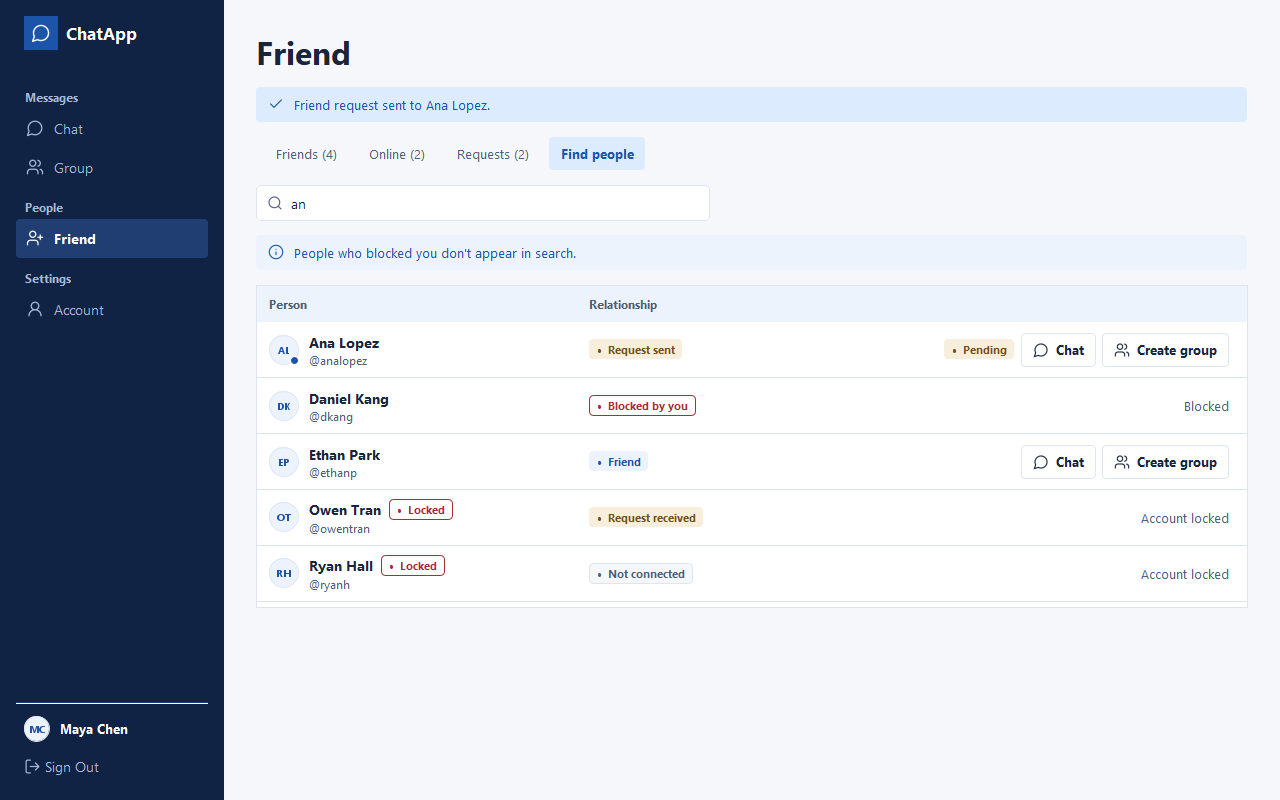
\includegraphics[width=.48\linewidth]{images/user-swing-find-people.png}\hfill
  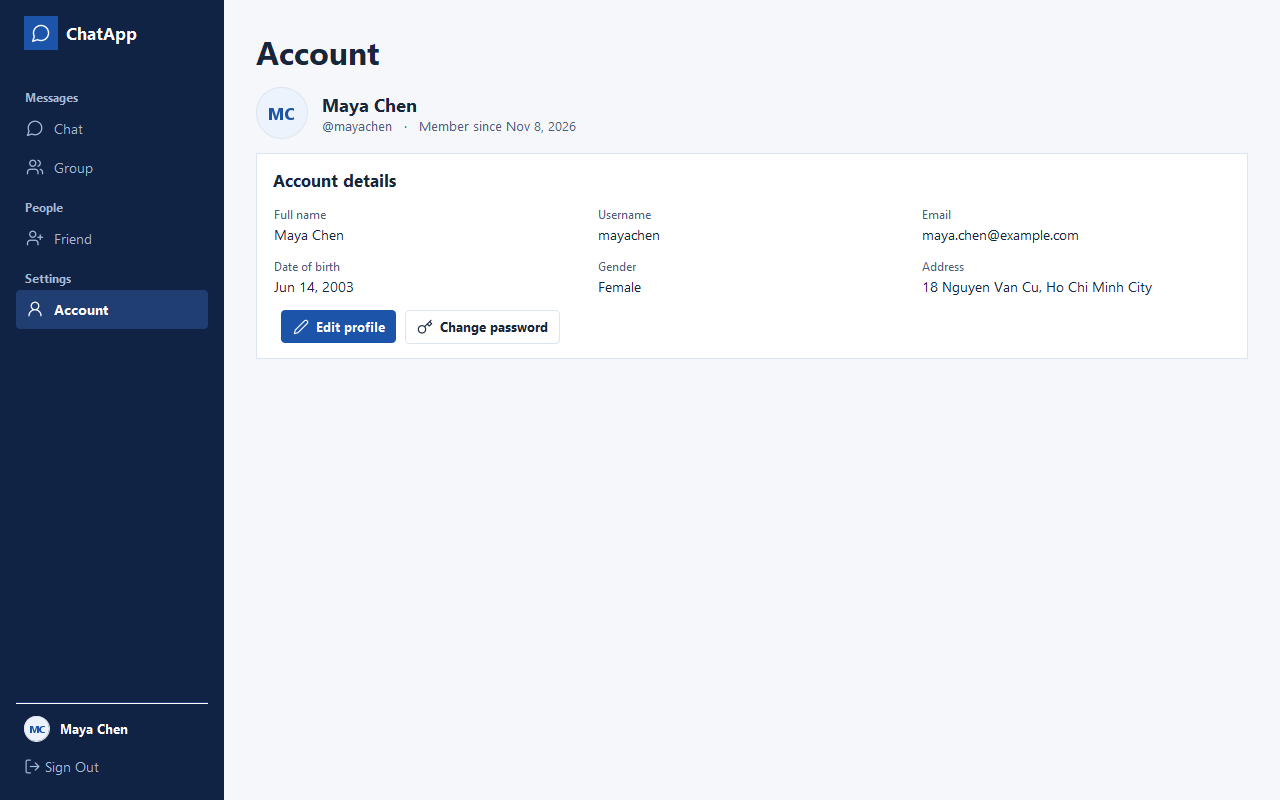
\includegraphics[width=.48\linewidth]{images/user-swing-account.png}
  \captionof{figure}{F09 and F03. Find people and send a friend request; the account profile.}
  \label{fig:user-swing-find-account}
\end{minipage}
